% latex foo.tex 
% dvips -Poutline -G0 foo.dvi -o 
% ps2pdf -dPDFSETTINGS#/prepress foo.ps
\documentclass[slidestop]{beamer}
\usepackage{fancyvrb}
\usepackage{hyperref}
%\usepackage{pstricks,pst-tree,pst-node,pst-plot,pst-3dplot}
\usepackage{graphicx}


\newcommand{\sect}[1]{
\section{#1}
\begin{frame}[fragile]\frametitle{#1}
}


\mode<presentation>
{
%  \usetheme{Madrid}
  % or ...

%  \setbeamercovered{transparent}
  % or whatever (possibly just delete it)
}

\usepackage[english]{babel}

\usepackage[latin1]{inputenc}

\title[Computer Graphics, CSCI 480]
{
Color
}

\subtitle{} % (optional)

\author[Geoffrey Matthews]
{Geoffrey Matthews}
% - Use the \inst{?} command only if the authors have different
%   affiliation.

\institute[WWU/CS]
{
  Department of Computer Science\\
  Western Washington University
}
% - Use the \inst command only if there are several affiliations.
% - Keep it simple, no one is interested in your street address.

\date{Fall 2012}

% If you have a file called "university-logo-filename.xxx", where xxx
% is a graphic format that can be processed by latex or pdflatex,
% resp., then you can add a logo as follows:

%\pgfdeclareimage[height=0.5cm]{university-logo}{WWULogoProColor}
%\logo{\pgfuseimage{university-logo}}

% If you wish to uncover everything in a step-wise fashion, uncomment
% the following command: 

%\beamerdefaultoverlayspecification{<+->}

\begin{document}

%\psset{arrowscale=2}

\begin{frame}
  \titlepage
\end{frame}

\newcommand{\mygraph}[2]{\centerline{\includegraphics[width=#1\textwidth]{#2}}}
\newcommand{\myref}[1]{\small\item\url{#1}}
\newcommand{\myreft}[1]{\footnotesize\item\url{#1}}

\sect{Online Resources}
{\bf Readings}
\begin{itemize}
\item \url{http://en.wikipedia.org/wiki/Color}
\item \url{http://en.wikipedia.org/wiki/CIE_1931_color_space}
\item \url{http://www.gelighting.com/na/business_lighting/spectral_power_distribution_curves/}

\end{itemize}

\end{frame}

%\begin{frame}
%  \frametitle{Outline}
%  \tableofcontents
%  % You might wish to add the option [pausesections]
%\end{frame}

\sect{Color spectrum}
\mygraph{1}{IMG_5026.JPG}
\end{frame}

\sect{Color spectrum}
\mygraph{1}{Linear_visible_spectrum.png}

\vfill
\begin{itemize}
\item Indigo is totally bogus:

\myref{http://blog.xkcd.com/2010/05/03/color-survey-results/}
\end{itemize}
\end{frame}

\sect{Outdoor light spectral power curve}
\mygraph{1}{outdoor_daylight.jpg}
\end{frame}

\sect{Incandescent spectral power curve}
\mygraph{1}{incandescent.jpg}
\end{frame}

\sect{Flourescent spectral power curve}
\mygraph{1}{SP65.jpg}
\end{frame}

\sect{Reflectance properties of objects}
\mygraph{.9}{lemonskin.png}
\begin{itemize}
\item Reflectance of lemon skin (pbrt book).
\end{itemize}
\end{frame}

\sect{Color functions in the eye}
\mygraph{.9}{CIE_eye_response.png}
\begin{itemize}
\item Three kinds of cones (color receptive neurons) in the retina.
\item Each overlaps the other two.  No pure stimulation of one kind.
  \item Blue/green distance greater than green/red.
\end{itemize}
\end{frame}

\sect{Tristimulus color space}
\mygraph{0.45}{Gamut_full.png}
\end{frame}

\sect{CIE XYZ colors}
\mygraph{0.6}{CIE_chromaticity.png}
\end{frame}

\sect{CIE RGB colors}
\mygraph{0.6}{CIE_RGB.png}
\end{frame}


\sect{Color cube}
\mygraph{0.6}{colorcube.png}
\end{frame}

\sect{Color cube RGB and CMY axes}
\mygraph{0.6}{colorcubeaxes.png}
\end{frame}

\sect{Additive and Subtractive Color}
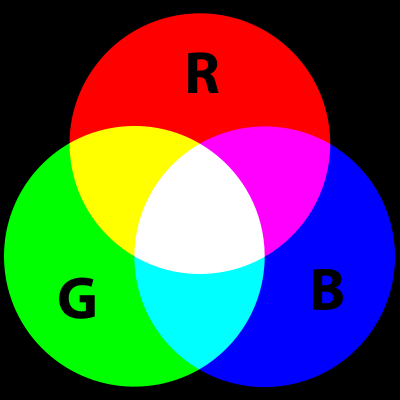
\includegraphics[width=0.5\textwidth]{400px-AdditiveColor.png}\hfill
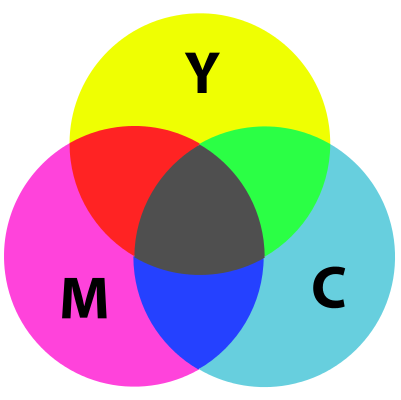
\includegraphics[width=0.5\textwidth]{SubtractiveColor.png}
\end{frame}

\sect{HSV and HSL models}
\mygraph{0.7}{hsl-hsv.png}
\end{frame}

\sect{Nervous system postprocessing}
\mygraph{.9}{orange-grey-illusion.png}
\end{frame}

\end{document}
